\documentclass[11pt,a4paper]{article}

\usepackage[a4paper,margin=2.5cm]{geometry}
\usepackage[spanish,es-nodecimaldot]{babel}
\usepackage[utf8]{inputenc}
\usepackage[T1]{fontenc}
\usepackage{lmodern}
\usepackage{amsmath,amssymb,mathtools}
\usepackage{booktabs}
\usepackage{graphicx}
\usepackage{caption}
\usepackage{microtype}
\usepackage{pdflscape}
\usepackage{hyperref}

\hypersetup{
  colorlinks=true,
  linkcolor=blue,
  urlcolor=blue,
  citecolor=blue,
  pdftitle={Polinomios y volúmenes de Ehrhart exactos en alta dimensión mediante contracción tensorial cilíndrica y reconstrucción por el teorema chino del resto}
}
\graphicspath{{./}}
\setlength{\emergencystretch}{2em}

\newcommand{\Ocal}{\mathcal{O}}
\newcommand{\Fp}{\mathbb{F}_p}
\newcommand{\Z}{\mathbb{Z}}
\newcommand{\Vol}{\operatorname{Vol}}

\title{Polinomios y volúmenes de Ehrhart exactos en alta dimensión mediante contracción tensorial cilíndrica y reconstrucción por el teorema chino del resto}
\author{Wendel León Alvarado}
\date{11 de noviembre de 2026}

\begin{document}
\maketitle

\begin{abstract}
Presentamos un algoritmo exacto para calcular conteos de Ehrhart,
polinomios $h^*$ de Ehrhart y volúmenes normalizados de politopos de orden
asociados con posets corona cilíndricos multicapa. El algoritmo contrae una
capa a la vez mediante sumas sufijas eje por eje sobre $\Fp$ y reconstruye
los conteos enteros mediante el teorema chino del resto (CRT). La cota exacta
por dilatación, $L_{k,n}(m)\leq(m+1)^{kn}$, determina cuántos primos de 61
bits son suficientes. La graduación del poset proporciona la simetría
palindrómica de $h^*$; por ello bastan la mitad independiente de los datos de
Ehrhart y una comprobación exacta adicional. La secuencia completa
$L_{k,n}(0),\ldots,L_{k,n}(kn)$ se evalúa después a partir del polinomio
reconstruido. El experimento cubre dimensiones de 6 a 40. En dimensión 40,
Tensor-CRT obtiene exactamente $7.8624\times10^{19}$ símplices en 43.355
segundos, con un pico de memoria de 52.84 MB medido mediante
\texttt{tracemalloc}; la enumeración directa de la triangulación unimodular
canónica alcanza el límite de 15 segundos.
\end{abstract}

\noindent\textbf{Palabras clave:}
polinomio de Ehrhart; politopo de orden; conteo exacto; contracción
tensorial; teorema chino del resto; cómputo en alta dimensión.

\section{Introducción}

El conteo exacto de puntos reticulares en politopos de alta dimensión suele
abordarse mediante una descomposición en conos o símplices. Para los
politopos de orden, la triangulación canónica es unimodular y está indexada
por las extensiones lineales del poset que los define. Esta es una línea
base exacta y conceptualmente sencilla, pero el número de símplices es el
número de extensiones lineales y puede crecer rápidamente. En nuestros
experimentos, enumerar esta descomposición tarda 14.069 segundos ya en
dimensión 16 y supera el límite de 15 segundos desde dimensión 20.

Estudiamos el poset corona cilíndrico $C_{k,n}$, con $k$ capas de $n$
vértices y dimensión $d=kn$. En vez de materializar la triangulación,
aprovechamos las relaciones de cubierta locales y contraemos un tensor de
frontera denso de dimensión $n$. La aritmética modular mantiene cada entrada
del tensor en un campo de 61 bits y el CRT recupera los enteros exactos.
Así, el espacio de trabajo no depende del número de símplices:
el algoritmo nunca almacena los $H_{k,n}(1)$ símplices.

Presentamos una batería de nueve instancias hasta $d=40$. El entorno no
disponía de los ejecutables Normaliz ni LattE \texttt{count}, ni del paquete
PyNormaliz; por tanto, no afirmamos haber medido tiempos directos con esas
herramientas. La línea base poliédrica que se informa aquí enumera
exactamente las extensiones lineales y se detiene a los 15 segundos. En las
instancias que alcanzan el límite, el conteo exacto de símplices se obtiene
independientemente del valor $H_{k,n}(1)$ calculado por Tensor-CRT.

\section{Definición del problema y datos de Ehrhart}

Para $k\geq2$ y $n\geq3$, sea
\[
  C_{k,n}=\{x_{j,i}:1\leq j\leq k,\ i\in\Z/n\Z\}
\]
con relaciones de cubierta
\[
  x_{j,i}\prec x_{j+1,i},
  \qquad
  x_{j,i}\prec x_{j+1,i+1}
  \quad (1\leq j<k),
\]
donde el segundo índice se interpreta cíclicamente. El politopo de orden
es
\[
  \Ocal(C_{k,n})=
  \{z\in[0,1]^{kn}:z_u\leq z_v\text{ siempre que }u\leq v\}.
\]
Es un politopo reticular de dimensión $d=kn$. Su conteo de Ehrhart y su
polinomio $h^*$ satisfacen
\begin{equation}
  L_{k,n}(m)=|m\Ocal(C_{k,n})\cap\Z^d|,
  \qquad
  \sum_{m\geq0}L_{k,n}(m)t^m
  =\frac{H_{k,n}(t)}{(1-t)^{d+1}},
  \qquad
  H_{k,n}(t)=\sum_{j=0}^{r}h_j^*t^j.
  \label{eq:ehrhart}
\end{equation}

El poset es graduado: toda cadena maximal tiene $k$ elementos. El grado
de su polinomio $h^*$ es, por tanto,
\[
  r=\deg H_{k,n}=d-k=k(n-1).
\]
El politopo de orden es Gorenstein, así que el polinomio $h^*$ es
palindrómico en su grado efectivo:
\begin{equation}
  h_j^*=h_{r-j}^*=h_{d-k-j}^*
  \quad (0\leq j\leq r).
  \label{eq:palindromic}
\end{equation}
El índice de simetría es $d-k-j$, no $d-j$, pues el grado es $d-k$.
Para cada instancia, el benchmark reconstruye por inversión triangular
la mitad independiente y comprueba la simetría con una muestra CRT exacta
adicional.

\section{Arquitectura algorítmica}

\subsection{Transferencia por capas cilíndricas}

Fijemos una dilatación $m$ y escribamos $N=m+1$. Cada capa es un vector
$a=(a_0,\ldots,a_{n-1})\in\{0,\ldots,m\}^n$. Definimos $F_1(a)=1$ y, para
$q\geq1$,
\begin{equation}
  F_{q+1}(a)=
  \sum_{b\in\{0,\ldots,m\}^n}
  \left(\prod_{i=0}^{n-1}
  \mathbf{1}\{a_i\leq b_i,\ a_i\leq b_{i+1}\}\right)F_q(b),
  \label{eq:transfer}
\end{equation}
con índices módulo $n$. Las dos desigualdades de cubierta imponen la cota
inferior
\[
  \ell_i(a)=\max(a_i,a_{i-1})
\]
para la coordenada $b_i$. Por consiguiente, la transición se escribe como
\begin{equation}
  F_{q+1}(a)=
  \sum_{\substack{b_i\geq\ell_i(a)\\0\leq i<n}}F_q(b).
  \label{eq:orthant}
\end{equation}
Después de $k-1$ transiciones,
\[
  L_{k,n}(m)=\sum_{a\in\{0,\ldots,m\}^n}F_k(a).
\]

Para un tensor $F$ indexado por $\{0,\ldots,m\}^n$, calculamos la suma
sufija multidimensional
\[
  S(t_0,\ldots,t_{n-1})
  =\sum_{b_0\geq t_0,\ldots,b_{n-1}\geq t_{n-1}}F(b).
\]
Se obtiene mediante un barrido sufijo unidimensional a lo largo de cada
eje. La transición queda entonces en
$F_{q+1}(a)=S(\ell_0(a),\ldots,\ell_{n-1}(a))$. Una suma directa sobre
pares de capas costaría $O(N^{2n})$ por transición; los barridos por eje y
la consulta indexada cuestan $O(nN^n)$. Los barridos, las consultas y las
reducciones se realizan módulo un primo $p$.

\subsection{Cotas CRT y reconstrucción exacta}

El conteo es no negativo y no supera el número de asignaciones posibles a
los $d$ vértices:
\begin{equation}
  0\leq L_{k,n}(m)\leq(m+1)^d.
  \label{eq:countbound}
\end{equation}
Si $p_1,\ldots,p_s$ son primos distintos de 61 bits y
$P=\prod_{\nu=1}^s p_\nu>(m+1)^d$, los residuos determinan de manera única
$L_{k,n}(m)$ en $[0,P)$. Una cota uniforme suficiente para todas las
dilataciones $0\leq m\leq d$ es
\[
  P>(d+1)^d=(d+1)^{kn}.
\]
La implementación utiliza la cota más ajustada por dilatación de
\eqref{eq:countbound}. Por ello, el número de primos informado es el máximo
requerido por las muestras independientes y no el número de primos de la
cota uniforme para el peor caso $m=d$.

Sea $r=d-k$. La identidad en base binomial derivada de
\eqref{eq:ehrhart} es
\begin{equation}
  L_{k,n}(m)=\sum_{j=0}^{\min(m,r)}
    h_j^*\binom{m+d-j}{d}.
  \label{eq:binomial}
\end{equation}
De ella se obtiene la recurrencia triangular
\begin{equation}
  h_m^*=L_{k,n}(m)-
  \sum_{j=0}^{m-1}h_j^*\binom{m+d-j}{d}.
  \label{eq:triangular}
\end{equation}
Calculamos los conteos CRT hasta $m=\lfloor r/2\rfloor+1$, aplicamos
\eqref{eq:triangular} a la primera mitad y usamos
\eqref{eq:palindromic} para los coeficientes restantes. La muestra extra
comprueba exactamente el coeficiente central de la simetría. Finalmente,
\eqref{eq:binomial} evalúa todos los conteos enteros
$L_{k,n}(0),\ldots,L_{k,n}(d)$. Por ello, no se requiere una contracción
tensorial independiente para cada uno de esos $d+1$ valores.

\subsection{Volúmenes y triangulación canónica}

La evaluación en uno es
\[
  H_{k,n}(1)=\sum_{j=0}^{r}h_j^*.
\]
En un politopo de orden, este valor también es el número de extensiones
lineales y, por tanto, el número de símplices unimodulares de la
triangulación canónica. Como cada símplice tiene volumen euclídeo $1/d!$,
\begin{equation}
  \Vol(\Ocal(C_{k,n}))=\frac{H_{k,n}(1)}{d!}.
  \label{eq:volume}
\end{equation}
Los volúmenes de la tabla se presentan como fracciones racionales exactas
reducidas.

\section{Complejidad y memoria}

Sea $N_{\max}$ uno más que la mayor dilatación CRT utilizada. Una
transición modular cuesta $O(nN_{\max}^n)$ operaciones de palabra: se
realizan $n$ barridos por eje y se calcula un índice con $O(n)$ operaciones
por entrada del tensor. Se repite para $k-1$ capas, a lo sumo $O(kn)$
dilataciones independientes y $O(\log M)$ primos, donde $M=(d+1)^d$ es la
cota uniforme del conteo. Como $N_{\max}\leq d+1=kn+1$, el trabajo de
contracción está acotado por
\[
  O\!\left(k^2n^2(kn+1)^n\log M\right),
\]
y, en particular, satisface la cota conservadora
\begin{equation}
  O\!\left(k^2n^3(kn+1)^n\log M\right).
  \label{eq:complexity}
\end{equation}
La inversión triangular de $h^*$ añade $O(d^2)$ operaciones enteras
exactas. Estas son cotas en el modelo de operaciones aritméticas; el costo
en bits también depende de los conteos exactos y los intermediarios CRT,
cuyas longitudes son $O(\log M)$ bits.

La implementación almacena los tensores de residuos actual y siguiente,
de tamaño $N_{\max}^n$, además de vectores de índices por bloques para la
consulta. El espacio de trabajo es $O(N_{\max}^n)$ palabras de máquina
(más los bits necesarios para representar los resultados enteros exactos)
y no es proporcional a $H_{k,n}(1)$. En particular, no se reserva una
lista de símplices. Una matriz densa de coordenadas de 64 bits para la
triangulación explícita requeriría
$H_{k,n}(1)(d+1)d\cdot8$ bytes; en $d=40$ esto equivale a
$1.0315\times10^{24}$ bytes, frente al pico medido de 52.84 MB mediante
\texttt{tracemalloc} para Tensor-CRT.

\section{Benchmark experimental hasta dimensión 40}

Todas las mediciones se produjeron con
\texttt{benchmark\_ehrhart\_d40.py}. El tiempo de Tensor-CRT incluye las
contracciones CRT independientes y la reconstrucción exacta del polinomio.
La memoria pico se mide con \texttt{tracemalloc} de Python. La columna
poliédrica corresponde a una enumeración recursiva exacta de extensiones
lineales, detenida después de 15 segundos. Un timeout es una observación
censurada $>15$ s, no un tiempo de línea base completado. En todas las filas,
el conteo exacto de símplices es $H_{k,n}(1)$, obtenido del numerador
exacto. Normaliz, LattE y PyNormaliz no estaban instalados en el entorno.

\begin{landscape}
\begin{center}
\captionsetup{hypcap=false}
\captionof{table}{Benchmark exacto de Tensor-CRT y de la triangulación
canónica. Los volúmenes son fracciones racionales reducidas.}
\label{tab:benchmark}
\small
\setlength{\tabcolsep}{4pt}
\renewcommand{\arraystretch}{1.15}
\resizebox{\linewidth}{!}{%
\begin{tabular}{@{}rrrrrrrl@{}}
\toprule
$(k,n)$ & $d$ & Primos CRT & Tensor-CRT (s) & Pico (MB) &
Línea base poliédrica & $H_{k,n}(1)$ & Volumen euclídeo exacto \\
\midrule
$(2,3)$ & 6  & 1 & 0.013 & 0.01 & 0.346 s & 48 & \texttt{1/15} \\
$(3,3)$ & 9  & 1 & 0.021 & 0.01 & 0.565 s & 384 & \texttt{1/945} \\
$(3,4)$ & 12 & 1 & 0.025 & 0.08 & 0.589 s & 50,688 & \texttt{1/9450} \\
$(4,4)$ & 16 & 1 & 0.062 & 0.25 & 14.069 s & 2,363,392 & \texttt{577/5108103000} \\
$(4,5)$ & 20 & 2 & 0.412 & 6.11 & \texttt{TIMEOUT $>15$ s} & 4,957,143,040 & \texttt{3782/1856156927625} \\
$(5,5)$ & 25 & 2 & 1.579 & 15.19 & \texttt{TIMEOUT $>15$ s} & 1,759,112,069,120 & \texttt{521/4593988395871875} \\
$(6,5)$ & 30 & 2 & 4.900 & 32.21 & \texttt{TIMEOUT $>15$ s} & 624,279,871,815,680 & \texttt{97921/41606059170426672796875} \\
$(7,5)$ & 35 & 3 & 17.339 & 40.00 & \texttt{TIMEOUT $>15$ s} & 221,547,727,526,297,600 & \texttt{6388/297940989719425403898421875} \\
$(8,5)$ & 40 & 3 & 43.355 & 52.84 & \texttt{TIMEOUT $>15$ s} & 78,624,058,898,424,791,040 & \texttt{615124/6383403244813084051148273014453125} \\
\bottomrule
\end{tabular}%
}
\end{center}
\end{landscape}

\begin{figure}[htbp]
  \centering
  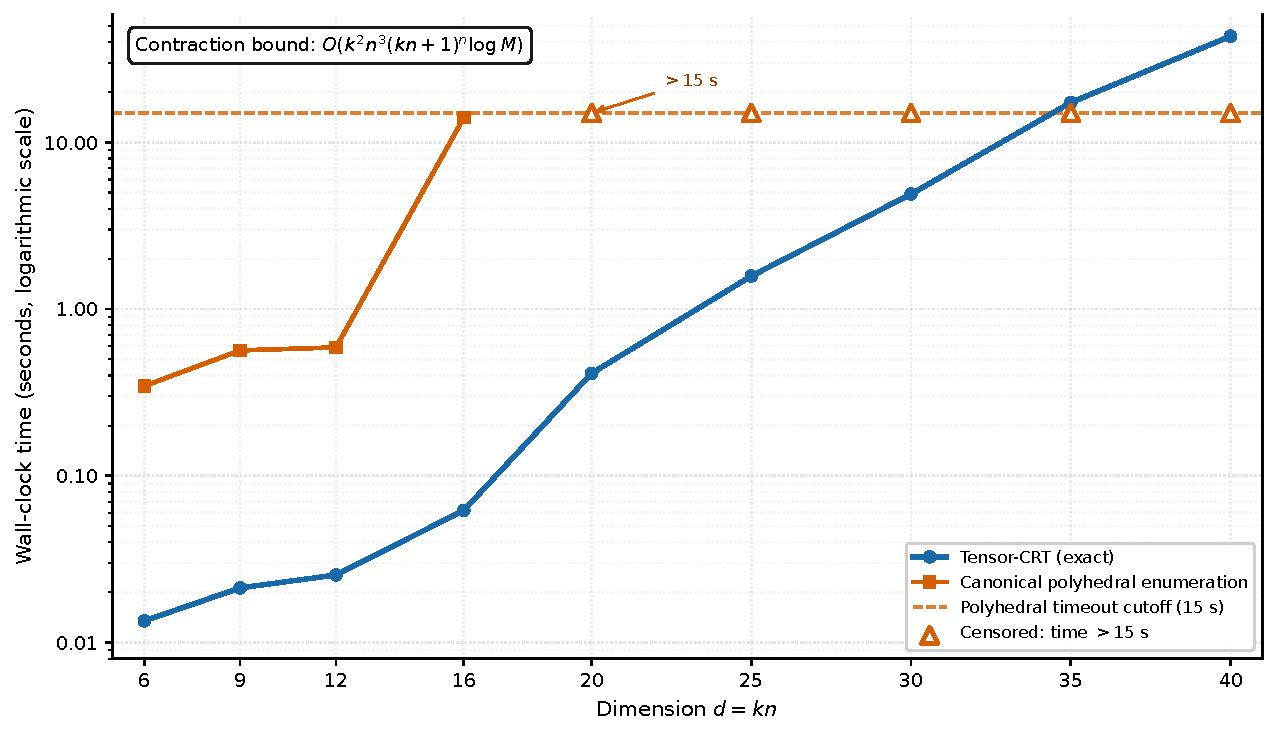
\includegraphics[width=0.94\linewidth]{fig_tiempos_d40.pdf}
  \caption{Comparación de tiempos de pared en escala logarítmica. Los
  triángulos indican que la enumeración poliédrica quedó censurada por el
  límite de 15 segundos. La anotación indica la cota asintótica de
  operaciones de Tensor-CRT.}
  \label{fig:times}
\end{figure}

\begin{figure}[htbp]
  \centering
  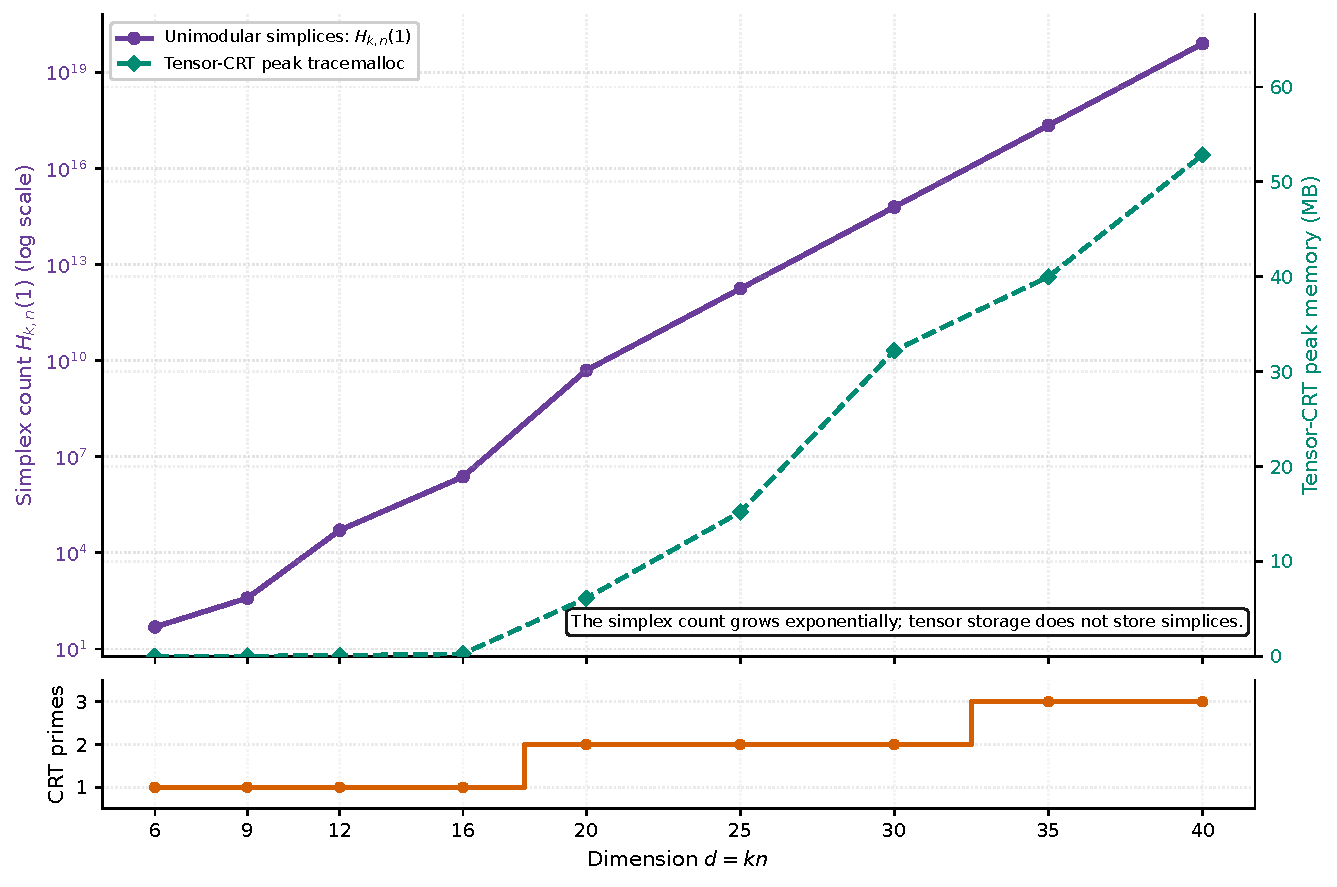
\includegraphics[width=0.94\linewidth]{fig_memoria_simplices_d40.pdf}
  \caption{Número exacto de símplices unimodulares canónicos, memoria pico
  de Tensor-CRT y número de primos CRT de 61 bits usados en las dilataciones
  independientes.}
  \label{fig:memory}
\end{figure}

La Figura~\ref{fig:times} muestra que la contracción tensorial exacta
completa los nueve casos, mientras que la enumeración directa de la
triangulación alcanza el límite desde $d=20$. La
Figura~\ref{fig:memory} muestra la diferencia entre el crecimiento rápido
del número de símplices y el espacio de trabajo tensorial: entre $d=6$ y
$d=40$, $H(1)$ aumenta de 48 a $7.8624\times10^{19}$, mientras que la
memoria pico medida aumenta de 0.01 MB a 52.84 MB. El máximo de primos CRT
necesarios para las muestras independientes es tres. Los vectores $h^*$
reportados son palindrómicos en grado $d-k$, y la muestra CRT exacta
adicional confirma esa simetría en cada instancia.

\section{Conclusión y reproducibilidad}

La contracción cilíndrica por capas sustituye la triangulación explícita
por sumas sufijas multidimensionales exactas, y el CRT transforma los
cálculos modulares acotados en datos enteros de Ehrhart. El benchmark
alcanza dimensión 40 sin que el espacio de trabajo tensorial se aproxime a
la memoria necesaria para almacenar explícitamente la triangulación.

La implementación, los datos del benchmark, el generador de figuras, las
figuras vectoriales y rasterizadas a 300 dpi y este manuscrito están en
\texttt{BENCHMARK\_D40/}. Las figuras se reproducen con
\texttt{python generar\_graficas.py}; este manuscrito se compila dos veces
con \texttt{pdflatex -interaction=nonstopmode -halt-on-error
paper\_tensor\_crt\_es.tex}. Una extensión natural consiste en sustituir el
patrón de cubiertas cilíndrico de dos vecinos por restricciones locales
sobre grafos periódicos más generales, conservando una frontera tensorial
de ancho acotado.

\begin{thebibliography}{9}
\bibitem{BeckRobins}
M. Beck y S. Robins,
\emph{Computing the Continuous Discretely: Integer-Point Enumeration in
Polyhedra}, 2.\textsuperscript{a} ed., Springer, 2015.

\bibitem{Stanley}
R. P. Stanley,
Two poset polytopes,
\emph{Discrete \& Computational Geometry} 1 (1986), 9--23.
\end{thebibliography}

\end{document}
